\documentclass[11pt]{article}
\usepackage[margin=1in]{geometry}                % See geometry.pdf to learn the layout options. There are lots.
\geometry{letterpaper}                   % ... or a4paper or a5paper or ... 
%\geometry{landscape}                % Activate for for rotated page geometry
%\usepackage[parfill]{parskip}    % Activate to begin paragraphs with an empty line rather than an indent
\usepackage[breaklinks=true, colorlinks=true, linkcolor=red, urlcolor=blue, citecolor=black]{hyperref}
\urlstyle{rm}
\usepackage{mathptmx}
\usepackage{graphicx}
\usepackage{amssymb}
\usepackage{epstopdf}
\usepackage{color}
\usepackage{sidecap}
\usepackage{authblk}
\usepackage{booktabs}
\usepackage[font=small,labelfont=bf]{caption}
\usepackage{enumitem}
\usepackage{wrapfig}
\DeclareGraphicsRule{.tif}{png}{.png}{`convert #1 `dirname #1`/`basename #1 .tif`.png}

\pagestyle{empty}

\def\bfr{\bf\color{red}}
\def\geohub{{\tt geohub}}
\def\selah{\emph{SELAH}}

%\title{\bf
%	Summary of SELAH Unsheltered Tract Recounts around\\ Echo Park Lake
%	}
%\author{}%,$\ddagger$
%
%\date{\today}                                           % Activate to display a given date or no date

\begin{document}
%\maketitle

\begin{center}
	\Large\bf Echo Park Homelessness May Have Risen Less Than It Seems 
	%Fall 2020 \selah\ Unsheltered Tract Recounts around Echo Park Lake

	\vspace{1ex}

	{\normalsize\rm Louis Abramson, PhD, for the \href{http://www.selahnhc.org}{\it SELAH Neighborhood Homeless Coalition} \\ \today}

%	\vspace{1em}

%	{\large\it Summary}	
\end{center}

\noindent {\bf Summary:} The number of tents near Echo Park Lake increased by over 100\% between 
January and October 2020. However, the total number of unsheltered {\it people} rose less dramatically. \selah\ 
data suggest that between 175 and 220 individuals lived exposed or in $\sim$150 informal dwellings in 
census tract 1975.00 as of last fall. Compared to the official \href{https://www.lahsa.org/data?id=45-2020-homeless-count-by-community-city}{LAHSA Point-In-Time (PIT) Count} of 174 
people, our preferred value of $\sim$190 residents would reflect a $\sim$9\% increase. While 
substantial, this modest rise reflects known COVID-related tent distribution efforts by local service 
providers, and is consistent with evidence suggesting that tent occupancy is down by perhaps 30\%
compared to the \href{https://www.lahsa.org/documents?id=4693-2020-greater-los-angeles-homeless-count-cvrtm-conversion-factors}{last SPA4 estimates}. More definitive statements are difficult, but our analysis suggests 
that, at a minimum, surveys establishing the fraction of tents not employed as dwellings will be key to 
obtaining an accurate assessment of today's unsheltered population.\\

\begin{figure*}[h]
	\centering
	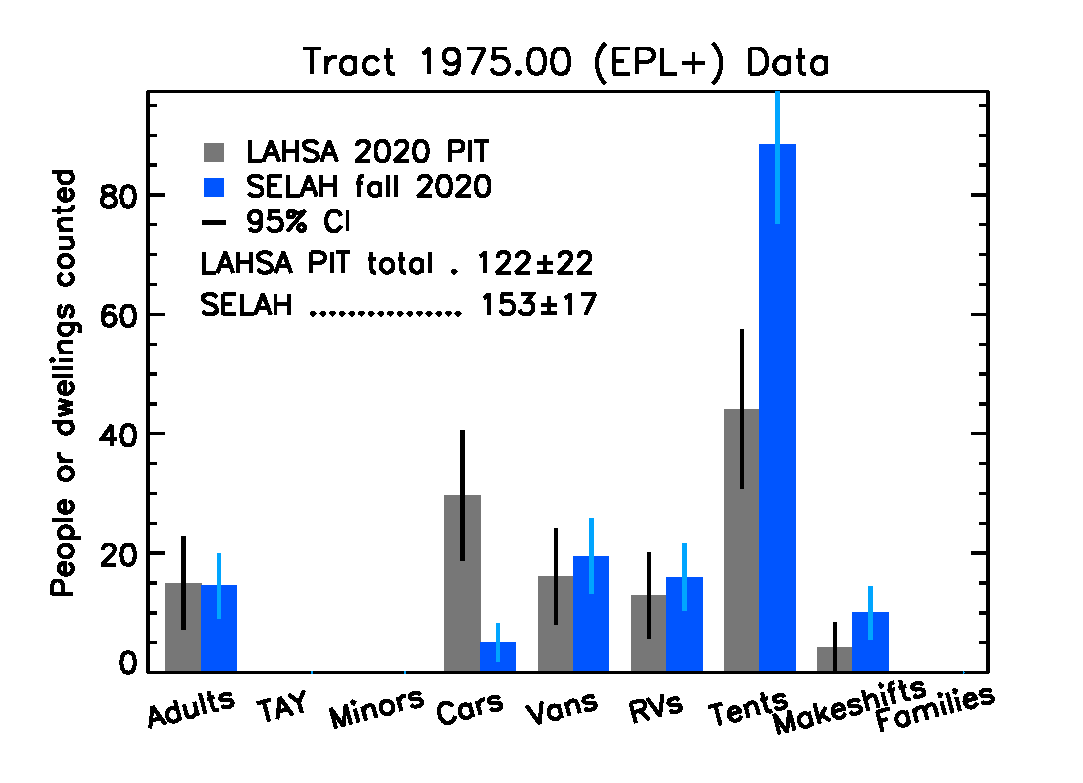
\includegraphics[width = 0.47\textwidth, trim = 1cm 0cm 0cm 1cm]{EPsummaryBars}
	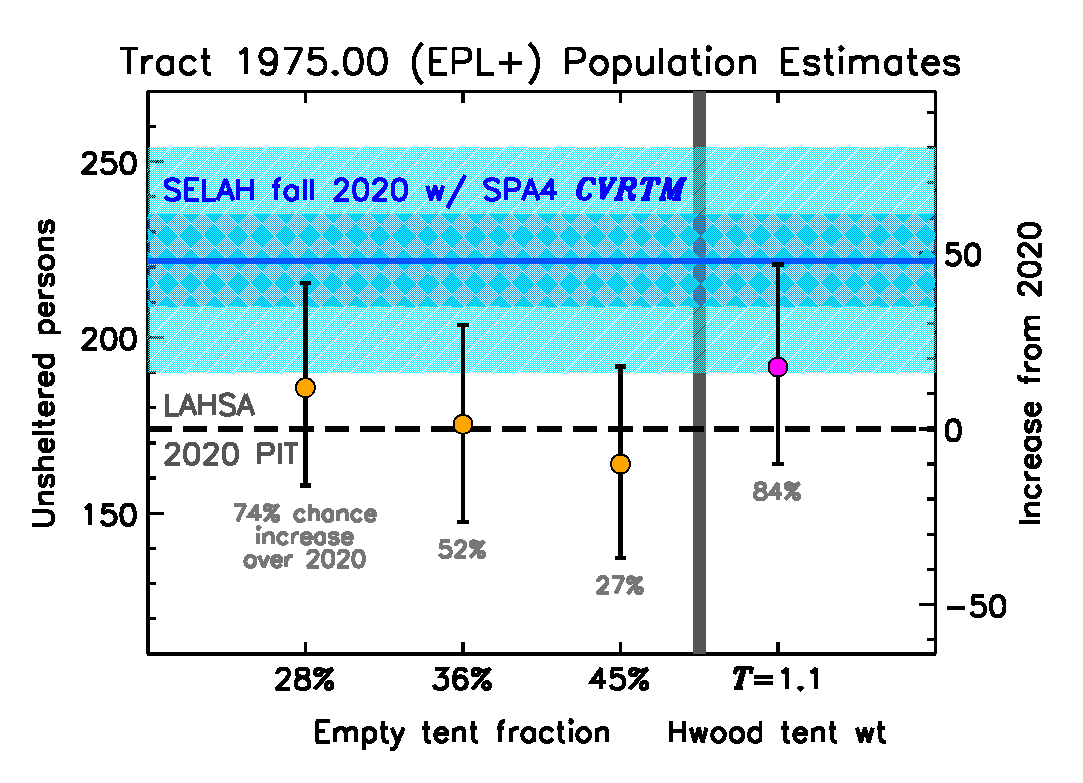
\includegraphics[width = 0.47\textwidth, trim = 1cm 0cm 0cm 1cm]{EPwEmpties}
	\caption{{\it Left:} \selah's recounts from fall 2020 (blue) compared to LAHSA PIT values
		from last January (grey). Car counts have fallen, but the 110\% rise in tents has a larger 
		impact on the population. 
		{\it Right:} combined with the official \href{https://www.lahsa.org/documents?id=4693-2020-greater-los-angeles-homeless-count-cvrtm-conversion-factors}{SPA4 2020 weights}, \selah's data imply 
		$220\pm30$ unsheltered people living near Echo Park lake (blue horizontal line + 
		bands; 90\% CI)---25\% more than 2020's official tally (horizontal dashes). 
		However, \selah\ outreach teams subsequently found $37\%\pm9\%$ of tents to 
		be unused for dwelling, implying a reduced rise of $\lesssim$10\% (yellow circles). 
		That value is consistent with estimates obtained by assuming tent occupancies 
		derived from data in Hollywood from 2021 (pink circle; $T=1.1$ people per tent).
		Estimates derived from the SPA4 weights ($T=1.45$ people per tent) may therefore be closer to 
		current upper limits. Percentages below each inference give the chance that the unsheltered 
		population increased compared to 2020.}
	\label{fig:results}
\end{figure*}

\begin{table*}[h!]
\caption{Tract 1975.00 Unsheltered Data}
\resizebox{\linewidth}{!}{%
\begin{tabular}{lcccccccccc}
\toprule
 & Adult & TAY & Unacc Minor & Car & Van & RV & Tent & Makeshift & Family & {\bf Total} \\ \cmidrule{1-11}
LAHSA Jan 2020 Counts & 15 & -- & -- & 30 & 16 & 13 & 44 & 4 & -- & {\bf 122} \\
SELAH Fall 2020 Counts & 14 & 0 & 0 & 5 & 19 & 16 & 88 & 10 & 0 & {\bf 153} \\ 
\bottomrule
\end{tabular}
}
\caption*{Counts are of objects and do not account for CVRTM weights.
All entries combined into LAHSA's ``Persons on the street'' category are listed as adults. 
\selah\ quantities reflect the average of survey results from 2 August and 18 October circa 11:00 AM.}
\label{tbl:rawData}
\end{table*}

\clearpage

\begin{wrapfigure}{r}{0.5\linewidth}
	\centering
	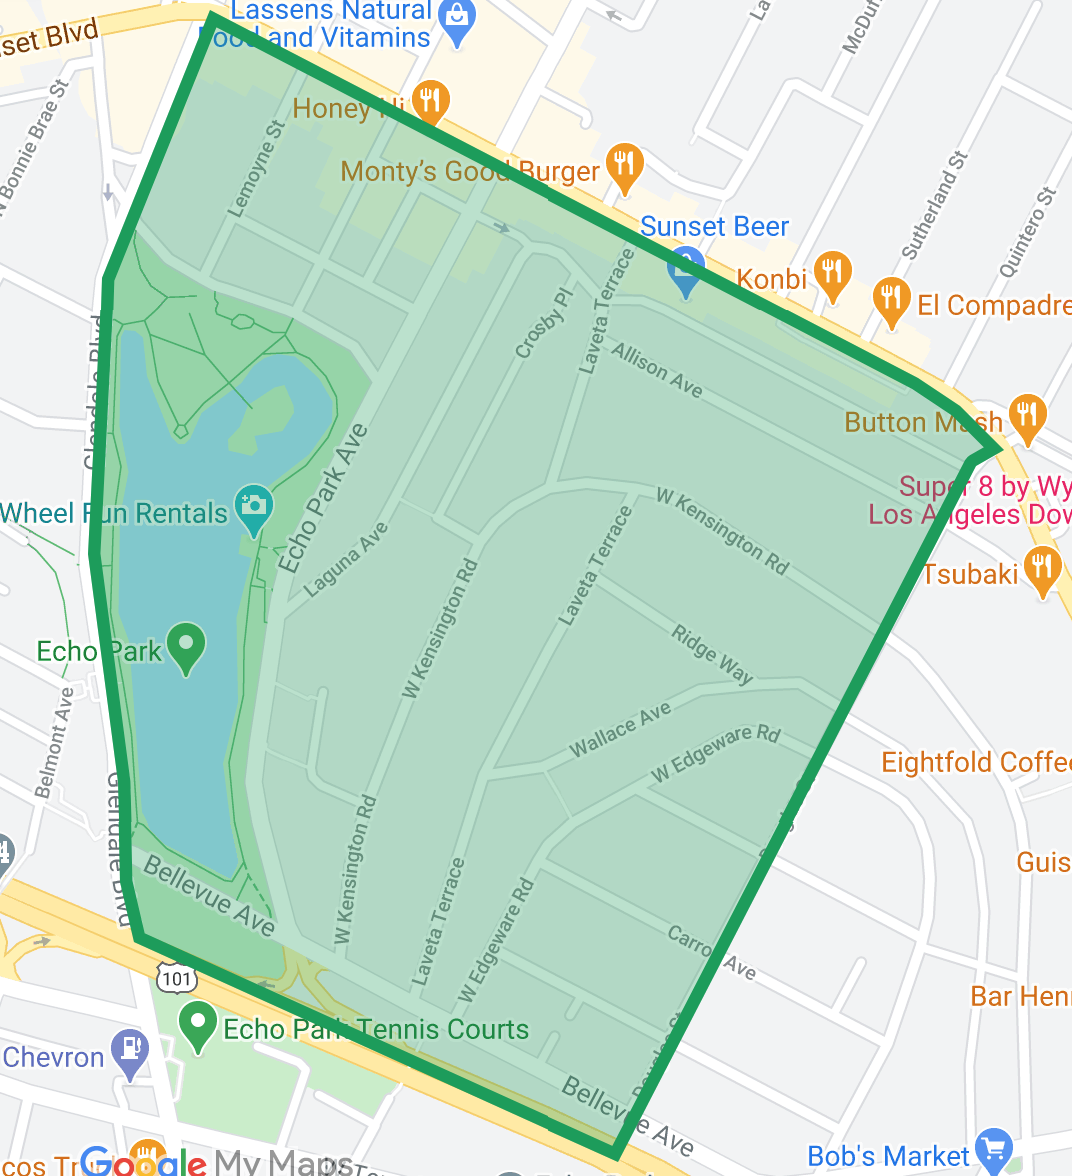
\includegraphics[width=\linewidth]{t1975}
	\caption{US Census tract 1975.00.}
	\label{fig:tract}
\end{wrapfigure}
\noindent {\bf Context:} \selah's outreach teams performed two recounts of US Census tract 1975.00 
on 2 August and 18 October 2020 (Figure \ref{fig:tract}). This tract contains Echo Park Lake and various 
CalTrans lands. The results of both surveys were statistically identical except for the estimate of vans, 
which rose from $14\pm3$ to $25\pm5$ between counts. Our final individual/dwelling statistics 
(Table \ref{tbl:rawData}) and total population estimates (Figure \ref{fig:results}) reflect the average 
of those assessments.\\


\noindent {\bf Results and uncertainties:} The population inferences in Figure \ref{fig:results} come 
from 10,000 Monte Carlo resamplings of the \selah\ survey data with counts perturbed by random 
draws from their Poisson error bars. In the cases of cars, vans, RVs, tents, and makeshift (CVRTM) 
dwellings, we additionally boosted counts by the relevant weighting factor perturbed by its error bar. 
In the baseline case---shown as blue horizontal bands in Figure \ref{fig:results}---we use the official 2020 
\href{https://www.lahsa.org/documents?id=4693-2020-greater-los-angeles-homeless-count-cvrtm-conversion-factors}{LAHSA SPA4 CVRTM weights}. The median result of that inference yields $220\pm30$ unsheltered 
individuals (90\% CI) compared to the PIT's estimate of 174 people.\\
\indent The CVRTM weights present systematic uncertainties, however, and so possible biases. 
For example, service providers have made a concerted effort to distribute tents during COVID, 
which might modulate $T$ downwards. (Other weights may have also shifted, but the fraction of 
tent-dwelling is such that changes to $T$ dominate the measurement error.) As such, multiplying by the 
2020 LAHSA tent weight may result in an overestimate of the actual unsheltered population.\\
\indent \selah\ cannot re-measure $T$ on large geographies, but two small-scale estimates 
suggest it has indeed fallen from the official 2020 value of 1.45 people per tent:
\begin{enumerate}
	\item \selah\ outreach teams surveyed 30 tents along Echo Park Lake's southern border on 21 
	February 2021, finding 11 of them to be used for storage or---based on statements from 
	neighbors or the team's weekly experience---abandoned. Albeit small, this sampling suggests that 
	up to 28\%--45\% of tents may be uninhabited (95\% CI) effectively reducing $T$ to 0.9.\footnote{
	Note: the official CVRTM weights are established using a 
	\href{https://www.lahsa.org/documents?id=4658-usc-2020-homeless-count-methodology-report}{methodology} that may not account for empty tents, and therefore may generally lead to overestimates of
	some degree.}
	\item Business Improvement District surveys of Hollywood conducted biweekly since January 2020 
	show the number of tents to have risen there faster than the number of visible individuals. Those
	data imply an average tent occupancy of $T=1.1\pm0.07$ people today.
\end{enumerate}
\noindent Using the lower unoccupied tent fraction in (1) to allow for inhabitants simply not being home, both 
modifications reduce our median unsheltered estimate to about 190 people---16 more than the 2020 PIT value.

\indent In all cases, further rigorous surveys---especially those aimed at understanding the fraction of
tents not used as  dwellings---are needed to ensure we understand the current scale of the 
homelessness crisis and plan accordingly.

%Lastly, \selah's tent count in tract 1975.00 is equivalent to over 130\% of LAHSA's PIT result for the {\it 
%entire} Echo Park Continuum of Care (CoC) last January (10 tracts; 67 tents). Scaling this tract's 2020 tent
%share by that value would imply a 110\% rise in unsheltered homelessness across the EP CoC since 2020. This would 
%correspond to $\sim$1250 people today---larger than Hollywood�s population. As such a rise seems unreasonable,
%it may be taken as further circumstantial evidence that tent occupancies have fallen, or as more direct evidence
%of internal migration within the EP CoC from other tracts into this.\\

\end{document}  